\begin{ex}%[2H5V2-2]
	Trong KG $Oxyz$, cho mặt cầu $(S)\colon (x-2)^2+(y-3)^2+(z-4)^2=14$ và mặt phẳng $(\alpha)\colon x+3 y+2 z-5=0$. Biết đường thẳng $\Delta$ nằm trong $(\alpha)$, cắt trục $Ox$ và tiếp xúc với $(S)$. Vec-tơ nào sau đây là vec-tơ chỉ phương của $\Delta$ ?
	\choice
	{$\vec{u}=(4 ;-2 ; 1)$}
	{\True $\vec{v}=(2 ; 0 ;-1)$}
	{$\vec{m}=(-3 ; 1 ; 0)$}
	{$\vec{n}=(1 ;-1 ; 1)$}
	\loigiai{
	Mặt cầu $(S)$ có tâm $I(2 ; 3 ; 4)$ và bán kính $R=\sqrt{14}$.\\
	Ta có $\mathrm{d}(I,(\alpha))=\sqrt{14}=R \Rightarrow(\alpha)$ tiếp xúc với $(S)$.\\
	Gọi $H$ là hình chiếu vuông góc của $I$ lên $(\alpha) \Rightarrow H(1 ; 0 ; 2)$.\\
	Gọi $A=\Delta \cap O x \Rightarrow A(a ; 0 ; 0)$ và $\overrightarrow{A H}=(a-1 ; 0 ;-2)$.\\
	Đường thẳng $\Delta$ nằm trong $(\alpha)$, cắt trục $O x$ và tiếp xúc với $(S)$ nên $\overrightarrow{A H} \perp \overrightarrow{n}_\alpha$.\\
	Tức là $a-1+0-4=0 \Leftrightarrow a=5 \Rightarrow \overrightarrow{AH}=(4 ; 0 ;-2)$ cùng phương với $\vec{v}=(2 ; 0 ;-1)$.}
\end{ex}

\begin{ex}%[2H5V3-2] 
	Trong không gian với hệ tọa độ $O x y z$, cho mặt phẳng $(P)\colon 2 x-2 y-z+9=0$ và mặt cầu $(S)\colon (x-3)^2+(y+2)^2+(z-1)^2=100$. Mặt phẳng $(P)$ cắt mặt cầu $(S)$ theo một đường tròn $(C)$. Tìm tọa độ tâm $K$ và bán kính $r$ của đường tròn $(C)$ là
	\choice
	{$K(3 ;-2 ; 1)$, $ r=10$}
	{\True $K(-1 ; 2 ; 3)$, $ r=8$}
	{$K(1 ;-2 ; 3)$, $r=8$}
	{$K(1 ; 2 ; 3)$, $r=6$}
	\loigiai{
		\begin{center}
			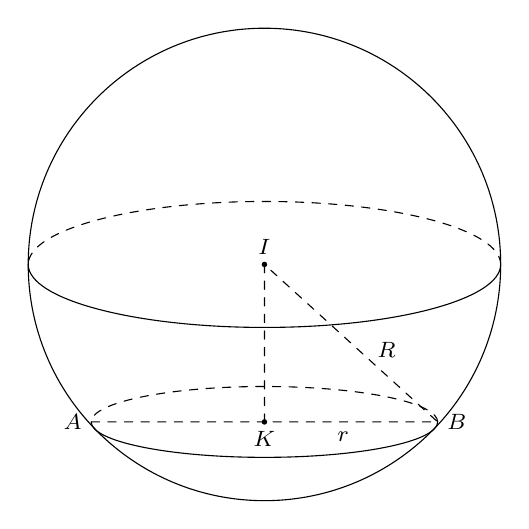
\begin{tikzpicture}[scale=1, font=\footnotesize, line join=round, line cap=round, >=stealth]
				\draw (0,0) circle (3);
				\draw[dashed] (3,0) arc [start angle=0,end angle=180,x radius=3,y radius=0.8];
				\draw (-3,0) arc [start angle=180,end angle=360,x radius=3,y radius=0.8];
				
				\draw[dashed] (2.2,-2) arc [start angle=0,end angle=180,x radius=2.2,y radius=0.45];
				\draw (-2.2,-2) arc [start angle=180,end angle=360,x radius=2.2,y radius=0.45];
				
				\draw (2.2,-2) node [right] {\footnotesize $B$};
				\draw (-2.2,-2) node [left] {\footnotesize $A$};
				\draw (0,0) node [above] {\footnotesize $I$};\fill (0,0) circle (1pt);
				\draw (1.55,-1.3) node [above] {\footnotesize $R$};
				\draw (1,-2) node [below] {\footnotesize $r$};
				\draw[dashed] (-2.2,-2)--(0,-2) (0,0)--(0,-2)--(2.2,-2)--(0,0);
				%Vẽ góc vuông
				\draw (0,-2) node [below] {\footnotesize $K$};\fill (0,-2) circle (1pt);
			\end{tikzpicture}
			
		\end{center}
		\begin{itemize}
			\item Mặt cầu $(S)$ có tâm $I(3 ;-2 ; 1) ; $ $R=10$.
			\item Khoảng cách từ $I$ đến $(P)$ là $I K=\mathrm{d} (I ;(P))=\dfrac{|6+4-1+9|}{3}=6$.
			\item Đường thẳng qua $I(3 ;-2 ; 1)$ vuông góc với $(P)$ có PTTS là $\heva{&x=3+2 t \\& y=-2-2 t \\& z=1-t.}$\\
			Khi đó, tọa độ tâm $K$ là nghiệm của hệ phương trình
			$$\heva{&x=3+2 t \\& y=-2-2 t \\& z=1-t \\& 2 x-2 y-z+9=0} \Rightarrow K(-1 ; 2 ; 3).$$
			\item  Bán kính $r=\sqrt{R^{2}-I K^{2}}=\sqrt{100-36}=8$.
		\end{itemize}
}\end{ex}

\begin{ex}%[2H5V3-4]
	Trong KG $Oxyz$, cho mặt phẳng $(P)\colon x-2y+2z-3=0$ và mặt cầu $(S)$ tâm $I(5;-3; 5)$, bán kính $R=2\sqrt{5}$. Từ một điểm $A$ thuộc mặt phẳng $(P)$ kẻ một đường thẳng tiếp xúc với mặt cầu $(S)$ tại $B$. Tính $OA$ biết $AB=4$.
	\choice
	{\True $OA=\sqrt{11}$}
	{$OA=5$}
	{$OA=3$}
	{$OA=\sqrt{6}$}
	\loigiai{
		Khoảng cách từ điểm $I$ đến mặt phẳng $(P)$ là $\mathrm{d}(I;(P))=\dfrac{|5-2\cdot(-3)+2\cdot 5-3|}{\sqrt{1^2+(-2)^2+2^2}}=6$.\\
		Ta có $AB$ tiếp xúc với $(S)$ tại $B$ nên tam giác $AIB$ vuông tại $B$, do đó ta có\\
		$IA=\sqrt{IB^2+AB^2}=\sqrt{R^2+AB^2}=\sqrt{(2\sqrt{5})^2+4^2}=6=d(I;(P)) \Rightarrow A$ là hình chiếu của $I$ lên $(P)$.\\
		Đường thẳng $IA$ đi qua điểm $I(5;-3; 5)$ có véc-tơ chỉ phương $\vec{u}=\overrightarrow{n}_(P)=(1;-2; 2)$ có phương trình $\heva{&x=5+t \\&y=-3-2t \\&z=5+2t.}$\\
		Ta có $A=IA\cap(P) \Rightarrow 5+t-2(-3-2t)+2(5+2t)-3=0\Rightarrow t=-2\Rightarrow A(3; 1; 1) \Rightarrow OA=\sqrt{11}$.}
\end{ex}

\begin{ex}%[2H5V3-4]
	Trong KG $Oxyz$, cho mặt cầu $(S)\colon x^2+y^2+z^2=9$ và điểm $M\left(x_0; y_0; z_0\right)$ thuộc $d\colon \heva{&x=1+t \\&y=1+2t \\&z=2-3t}$. Ba điểm $A$, $B$, $C$ phân biệt cùng thuộc mặt cầu sao cho $MA$, $MB$, $MC$ là tiếp tuyến của mặt cầu. Biết rằng mặt phẳng $(ABC)$ đi qua điểm $D(1; 1; 2)$. Tổng $T=x_0^2+y_0^2+z_0^2$ bằng
	\choice
	{$30$}
	{\True $26$}
	{$20$}
	{$21$}
	\loigiai{
		Mặt cầu $(S)$ có tâm $O(0; 0; 0)$ và bán kính $R=3$. Gọi $M\left(1+t_0; 1+2t_0; 2-3t_0\right) \in d$.\\
		Giả sử $T(x; y; z) \in(S)$ là một tiếp điểm của tiếp tuyến $MT$ với mặt cầu $(S)$. Khi đó 
		$$
		\begin{aligned}
			&OT^2+MT^2=OM^2\\
			& \Leftrightarrow 9+\left[x-\left(1+t_0\right)\right]^2+\left[y-\left(1+2 t_0\right)\right]^2+\left(z-\left(2-3 t_0\right)\right)^2=\left(1+t_0\right)^2+\left(1+2 t_0\right)^2+\left(2-3 t_0\right)^2 \\
			& \Leftrightarrow\left(1+t_0\right) x+\left(1+2 t_0\right)+\left(2-3 t_0\right) z-9=0.
		\end{aligned}
		$$
		Suy ra phương trình mặt phẳng $(ABC)$ có dạng $\left(1+t_0\right) x+\left(1+2t_0\right) y+\left(2-3t_0\right) z-9=0$.
		Do $D(1; 1; 2) \in(ABC)$ nên $1+t_0+1+2t_0+2.(2-3t)-9=0\Leftrightarrow t_0=-1\Rightarrow M(0;-1; 5)$.\\
		Vậy $T=0^2+(-1)^2+5^2=26$.
	}
\end{ex}

\begin{ex}%[2H5V1-7] 
	Trong KG $Oxyz$ cho hai điểm $A(0 ; 0 ; 3)$, $B(-2 ; 0 ; 1)$ và mặt phẳng $(\alpha)\colon 2 x-y+2 z+8=0$. Hỏi có bao nhiêu điểm $C$ trên mặt phẳng $(\alpha)$ sao cho tam giác $ABC$ đều?
	\choice
	{$2$}
	{$1$}
	{\True $0$}
	{Vô số}
	\loigiai{
		Gọi $(P)$ mặt phẳng trung trực của $A B$, khi đó phương trình của $(P)$ là $x+z-1=0$.\\
		Ta có $\overrightarrow{n}_P=(1 ; 0 ; 1),$ $ \overrightarrow{n}_{\alpha}=(2 ;-1 ; 2)$ nên $\left[\overrightarrow{n}_P, \overrightarrow{n}_{\alpha}\right]=(1 ; 0 ;-1)$.\\
		Gọi $d$ là giao tuyến của mặt phẳng $(P)$ với mặt phẳng $(\alpha)$. Chọn $\overrightarrow{u}_d=(1 ; 0 ;-1)$
		và điểm $M(1 ; 10 ; 0) \in d$ nên PTTS của $d$ là $\heva{&x=1+t \\& y=10 \\& z=-t.}$\\
		Do tam giác $A B C$ đều nên $C A=C B$ hay $C$ thuộc mặt phẳng trung trực của $A B$, mà $C \in(\alpha)$ nên $C \in(P) \cap(\alpha)=d$ suy ra tọa độ $C$ có dạng $C(1+t ; 10 ;-t)$.\\
		Do $\triangle A B C$ đều nên $A C=A B$, thay tọa độ các điểm ta có
		\allowdisplaybreaks
		\begin{eqnarray*}
			&&\sqrt{(1+t-0)^2+(10-0)^2+(-t-3)^2}=\sqrt{(-2-0)^2+(0-0)^2+(1-3)^2} \\&\Leftrightarrow& t^2+4 t+51=0\left(^{*}\right)
		\end{eqnarray*}
		Do phương trình $\left(^{*}\right)$ vô nghiệm nên không tồn tại điểm $C$ thỏa mãn yêu cầu bài toán.
		
}\end{ex}

\begin{ex}%[2H5V3-4] 
	Trong KG $Oxyz$, cho mặt cầu $(S)$ tâm $I(1 ; 3 ; 9)$ bán kính bằng $3$. Gọi $M$, $ N$ là hai điểm lần lượt thuộc hai trục $Ox$, $Oz$ sao cho đường thẳng $M N$ tiếp xúc với $(S)$, đồng thời mặt cầu ngoại tiếp tứ diện $OIMN$ có bán kính bằng $\dfrac{13}{2}$. Gọi $A$ là tiếp điểm của $M N$ và $(S)$, giá trị $A M \cdot A N$ bằng
	\choice
	{$39$}
	{\True $12 \sqrt{3}$}
	{$18$}
	{$28 \sqrt{3}$}
	\loigiai{
		\begin{itemize}
			\item Đặt $M(a ; 0 ; 0)$ và $N(0 ; 0 ; b)$. \\Nhận xét: $(S)$ tiếp xúc $(O x z)$ mà $M N \subset(O x z)$ tiếp xúc $(S)$ nên $M N$ tiếp xúc $(S)$ tại tiếp điểm của $(S)$ và $(O x z) \Rightarrow A(1 ; 0 ; 9)$.
			\item $\heva{&\overrightarrow{A M}=(a-1 ; 0 ;-9) \\& \overrightarrow{A N}=(-1 ; 0 ; b-9)} \Rightarrow \dfrac{a-1}{-1}=\dfrac{-9}{b-9} \Rightarrow(a-1)(b-9)=9$.
			\item Khi đó $O I M N$ có $\triangle O M N$ vuông tại $O,$ $(I M N) \perp(O M N)$ (do $I A \subset(I M N),$ $ I A \perp(O M N)$), suy ra bán kính mặt cầu ngoại tiếp $O I M N$ bằng bán kính đường tròn ngoại tiếp $\triangle I M N$ bằng $\dfrac{13}{2}$.\\
			Suy ra $\dfrac{1}{2} \cdot 3 \cdot M N=\dfrac{I M \cdot I N \cdot M N}{4 \cdot \dfrac{13}{2}} \Leftrightarrow I M \cdot I N=39$.\hfill(1)\\
			Mà 
			\allowdisplaybreaks
			\begin{eqnarray*}
				I M&=&\sqrt{(a-1)^2+3^2+9^2}=\sqrt{(a-1)^2+90}.\\
				I N&=&\sqrt{1^2+3^2+(b-9)^2}=\sqrt{10+\dfrac{81}{(a-1)^2}}.
			\end{eqnarray*}
			Thay vào (1) ta được
			$$\left[(a-1)^2+90\right]\left[10+\dfrac{81}{(a-1)^2}\right]=1521 \Leftrightarrow(a-1)^2=27.$$
			Ta có $\heva{&A M=\sqrt{(a-1)^2+81}=\sqrt{108}=6 \sqrt{3} \\& A N=\sqrt{1+(b-9)^2}=\sqrt{1+3}=2} \Rightarrow A M \cdot A N=12 \sqrt{3}$.
			
		\end{itemize}
}\end{ex}
\begin{ex}%[2H5V3-4] 
	Trong không gian $O x y z$, cho mặt cầu $(S)$ tâm $I(4 ; 1 ; 2)$ bán kính bằng $2$. Gọi $M$; $N$ là hai điểm lần lượt thuộc hai trục $O x$; $O y$ sao cho đường thẳng $M N$ tiếp xúc với $(S)$, đồng thời mặt cầu ngoại tiếp tứ diện $O I M N$ có bán kính bằng $\dfrac{7}{2}$. Gọi $A$ là tiếp điểm của $M N$ và $(S)$, giá trị $A M \cdot A N$ bằng
	\choice
	{\True $6 \sqrt{2}$}
	{$14$}
	{$8$}
	{$9 \sqrt{2}$}
	\loigiai{
		\begin{itemize}
			\item \textbf{Cách 1:}\\
			Ta có $\mathrm{d} (I,(O x y))=2$ nên mặt cầu $(S)$ tiếp xúc với mặt phẳng $(O x y)$ tại điểm $A(4 ; 1 ; 0)$, đồng thời đường thẳng $M N$ tiếp xúc với $(S)$ cũng tại điểm $A(4 ; 1 ; 0)$ do $M N \subset(O x y)$.\\
			Gọi $M(m ; 0 ; 0) ;$ $ N(0 ; n ; 0),$ $ m,$ $ n>0$.\\
			Do $A \in M N$ nên 
			\allowdisplaybreaks
			\begin{eqnarray*}
				{A M}=k \overrightarrow{A N} &\Rightarrow&\heva{&m-4=-4 k \\& -1=k(n-1)} \Rightarrow(m-4)(n-1)=4 \\&\Leftrightarrow& m=\dfrac{4 n}{n-1}, n-1 \neq 0.
			\end{eqnarray*}
			Phương trình mặt phẳng trung trực đoạn $O I\colon 4 x+y+2 z-\dfrac{21}{2}=0$.\\
			Phương trình mặt phẳng trung trực đoạn $O M\colon  x=\dfrac{m}{2}$.\\
			Phương trình mặt phẳng trung trực đoạn $O N\colon  y=\dfrac{n}{2}$.\\
			Do đó tâm mặt cầu ngoại tiếp tứ diện $O I M N$ là $J\left(\dfrac{m}{2} ; \dfrac{n}{2} ; \dfrac{-n^{2}+6 n-21}{4 n-4}\right)$.\\
			Theo giả thuyết cầu ngoại tiếp tứ diện $O I M N$ có bán kính bằng $\dfrac{7}{2}$ nên $O J=\dfrac{7}{2}$
			\allowdisplaybreaks
			\begin{eqnarray*}
				&\Leftrightarrow& O J^2=\dfrac{49}{4}\\&\Leftrightarrow& \dfrac{4 n^2}{(n-1)^2}+\dfrac{n^2}{4}+\dfrac{\left(n^2-6 n+21\right)^2}{16(n-1)^2}=\dfrac{49}{4}\\&\Leftrightarrow& n^{4}-4 n^{3}-10 n^2+28 n+49=0\\&\Leftrightarrow& n=1 \pm 2 \sqrt{2}.
			\end{eqnarray*}
			Vì $n>0$ nên chọn $n=1+2 \sqrt{2}$, suy ra $m=4+\sqrt{2}$.\\
			Khi đó $A M \cdot A N=6 \sqrt{2}$.
			\item \textbf{Cách 2:}\\
			Dễ thấy mặt cầu $(S)$ tiếp xúc với mặt phẳng $(O x y)$ tại điểm $A(4 ; 1 ; 0)$, đồng thời đường thẳng $M N$ tiếp xúc với $(S)$ cũng tại điểm $A(1 ; 4 ; 0)$ do $M N \subset(O x y)$.\\
			Gọi $M(a ; 0 ; 0) ; $ $N(0 ; b ; 0)$.\\
			Do $A \in M N$ nên $\overrightarrow{A M}=k \overrightarrow{A N} \Rightarrow\heva{&a-4=-4 k \\& -1=k(b-1)} \Rightarrow \dfrac{1}{b}+\dfrac{4}{a}=1$.\\
			Gọi $J$ là trung điểm $M N \Rightarrow J\left(\dfrac{a}{2} ; \dfrac{b}{2} ; 0\right)$ và $I(4 ; 1 ; 2)$ thuộc đường thẳng $\Delta$ vuông góc với $(O x y)$ tại điểm $J$. Phương trình $\Delta$ là $\heva{&x=\dfrac{a}{2} \\& y=\dfrac{b}{2} \\& z=t.}$\\
			Suy ra tâm của mặt cầu ngoại tiếp tứ diện $OIMN$ là điểm $K\left(\dfrac{a}{2} ; \dfrac{b}{2} ; t\right)$.\\
			Theo giả thiết ta có hệ 
			\allowdisplaybreaks
			\begin{eqnarray*}
				&&\heva{&\dfrac{1}{b}+\dfrac{4}{a}=1 \\& O K=\dfrac{7}{2} \\& I K=\dfrac{7}{2}} \Leftrightarrow \heva{&\dfrac{1}{b}+\dfrac{4}{a}=1 \\& \dfrac{a^2}{4}+\dfrac{b^2}{4}+t^2=\dfrac{49}{4} \\& \left(\dfrac{a}{2}-4\right)^2+\left(\dfrac{b}{2}-1\right)^2+(t-2)^2=\dfrac{49}{4}}\\&\Leftrightarrow&\heva{&a=\dfrac{4 b}{b-1} \\& 4 a+b+4 t-21=0 \\& \dfrac{a^2}{4}+\dfrac{b^2}{4}+t^2=\dfrac{49}{4}} \Leftrightarrow\heva{&a=\dfrac{4 b}{b-1} \\& t=\dfrac{b^2-6 b+21}{4(b-1)} \\& \dfrac{a^2}{4}+\dfrac{b^2}{4}+t^2=\dfrac{49}{4}}
				\\&\Rightarrow& \dfrac{b^2}{4}+\dfrac{4 b^2}{(b-1)^2}+\dfrac{\left(b^2-6 b+21\right)^2}{16(b-1)^2}=\dfrac{49}{4} \\&\Leftrightarrow& 4 b^2+64\left(1+\dfrac{1}{b-1}\right)^2+\left(b-5+\dfrac{16}{b-1}\right)^2=196
				\\&\Leftrightarrow& 4 b^2+64+\dfrac{128}{b-1}+\dfrac{64}{(b-1)^2}+(b-5)^2+32(b-5) \cdot \dfrac{1}{b-1}+\dfrac{256}{(b-1)^2}=196
				\\&\Leftrightarrow& 5 b^2-10 b+25+\dfrac{320}{(b-1)^2}+32(b-5+4) \cdot \dfrac{1}{b-1}=132 \\&\Leftrightarrow&(b-1)^2+\dfrac{64}{(b-1)^2}=16
				\Leftrightarrow\left[(b-1)^2-8\right]^2=0 \Leftrightarrow(b-1)^2=8 \\&\Leftrightarrow&\hoac{&b=1-2 \sqrt{2} \\& b=1+2 \sqrt{2}.}
			\end{eqnarray*}
			\begin{itemize}
				\item Với $b=1-2 \sqrt{2}$ ta được $a=4-\sqrt{2} \Rightarrow A M \cdot A N=6 \sqrt{2}$.
				\item Với $b=1+2 \sqrt{2}$ ta được $a=4+\sqrt{2} \Rightarrow A M \cdot  A N=6 \sqrt{2}$.
			\end{itemize}
		\end{itemize}
}\end{ex}

\Closesolutionfile{ans}
\indapan{10}{ans/ans-C5B3CD4_1-10-D3-LC}
\Opensolutionfile{ans}[ans/C5B3CD4_22-31-kq]
\TNSA
\begin{ex}%[2H5V3-4] 
	Trong không gian với hệ trục $Oxyz$, cho mặt cầu $(S)\colon  x^2+y^2+z^2-2 x-4 y+6 z-13=0$ và đường thẳng $d\colon  \dfrac{x+1}{1}=\dfrac{y+2}{1}=\dfrac{z-1}{1}$. Điểm $M(a ; b ; c),$ $(a>0)$ nằm trên đường thẳng $d$ sao cho từ $M$ kẻ được ba tiếp tuyến $M A, $ $M B,$ $ M C$ đến mặt cầu $(S)$ $(A,$ $ B,$ $ C$ là các tiếp điểm) và $\widehat{A M B}=60^{\circ},$ $ \widehat{BMC}=60^{\circ},$ $ \widehat{CMA}=120^{\circ}$. Biết $a^3+b^3+c^3=\dfrac{m}{n}$, tính $m+n$.
	\shortans[]{$121$}
	\loigiai{
		\begin{center}
			\begin{tikzpicture}[scale=1]
				\coordinate [label=left:$I$](I) at (0,0);
				\pgfmathsetmacro\a{sqrt(2.75)}
				\coordinate [label=above right:$A$](A) at (2.5,\a);
				\coordinate [label=below right:$C$](C) at (2.5,-\a);
				\coordinate (I') at ($(A)!1!90:(I)$);
				\draw (0,0) circle (3);
				\coordinate (J) at 
				(5,0);
				%gIAO ĐIỂM M
				\draw[name path=done,color=white] (I)--(J);
				\draw[name path=dtwo,color=white] (A)--(I');
				\path [name intersections={of=done and dtwo,by=M}];
				\draw (M) node[below right]{$M$};
				%gIAO ĐIỂM H
				\draw[name path=a] (I)--(M);
				\draw[name path=b] (A)--(C);
				\path [name intersections={of=a and b,by=H}];
				\draw (H) node[below left]{$H$};
				\foreach \diem in {A,I,C,M,H}	\fill (\diem)circle(1.5pt);		
				\draw[smooth](I)--(A)--(M)--(C)--(I);
				%	\draw[dashed](B)--(D);
			\end{tikzpicture}
		\end{center}
		Mặt cầu $(S)$ có tâm $I(1 ; 2 ;-3)$ và bán kính $R=\sqrt{1^2+2^2+(-3)^2+13}=3 \sqrt{3}$.\\
		Gọi $(C)$ là đường tròn giao tuyến của mặt phẳng $(A B C)$ và mặt cầu $(S)$.\\
		Đặt $M A=M B=M C=x$ khi đó $A B=x ;$ $ B C=x \sqrt{2} ; $ $C A=x \sqrt{3}$ do đó tam giác $A B C$ vuông tại $B$ nên trung điểm $H$ của $A C$ là tâm đường tròn $(C)$ và $H,$ $ I,$ $ M$ thẳng hàng.\\
		Vì $\widehat{AMC}=120^{\circ}$ nên tam giác $A I C$ đều do đó $x \sqrt{3}=R \Leftrightarrow x=3$ suy ra $I M=2 A M=2 x=6$.\\
		Lại có $M \in d$ nên $M(-1+t ;-2+t ; 1+t),$ $(t>1)$ mà $I M=6$ nên 
		\allowdisplaybreaks
		\begin{eqnarray*}
			(t-2)^2+(t-4)^2+(t+4)^2=36\Leftrightarrow 3 t^2-4 t=0 \Leftrightarrow \hoac{&t=0 \\& t=\dfrac{4}{3}.}
		\end{eqnarray*}
		Mà $a>0$ nên $t=\dfrac{4}{3}$ suy ra $H\left(\dfrac{1}{3} ;-\dfrac{2}{3} ; \dfrac{7}{3}\right)$. Vậy $a^3+b^3+c^3=\dfrac{112}{9}=\dfrac{m}{n}$.\\
		Khi đó $m+n=121$.
}\end{ex}

\begin{ex}%[2H5V3-4] 
	Trong không gian $O x y z$, cho mặt cầu $(S)$ tâm $I(1 ; 4 ; 2)$, bán kính bằng $2$. Gọi $M,$ $ N$ là hai điểm lần lượt thuộc hai trục $O x$, $ O y$ sao cho đường thẳng $M N$ tiếp xúc với $(S)$, đồng thời mặt cầu ngoại tiếp tứ diện $O I M N$ có bán kính bằng $\dfrac{7}{2}$. Gọi $A$ là tiếp điểm của $M N$ và $(S)$, tính giá trị $A M \cdot A N$ (làm tròn đến hàng phần trăm).
	\shortans[]{$8{,}48$}
	\loigiai{
		\begin{center}
			\begin{tikzpicture}[scale=1, line join=round, line cap=round, >=stealth]
				\coordinate [label=below:$O$](O) at (0,0);
				\coordinate [label=above right:$M$](M) at (5,0);
				\coordinate [label=below:$N$](N) at (-3,-2);
				\coordinate [label=above:$I$](I) at (2,4);
				\coordinate [label=below:$A$](A) at ($(N)! .75 ! (M)$);
				%gIAO ĐIỂM P
				\draw[name path=done] (I)--(N);
				\draw[name path=dtwo,color=white] (O)--($(O)! 1.5 ! (0,3)$);
				\path [name intersections={of=done and dtwo,by=P}];
				\draw[->] (M)--($(O)! 1.5 ! (M)$) node[below]{$x$};	
				\draw[->] (P)--($(O)! 3 ! (P)$) node[right]{$z$};	
				\draw[->] (N)--($(O)! 1.5 ! (N)$) node[below right]{$y$};	
				\foreach \diem in {O,M,N,I,A}	\fill (\diem)circle(1.5pt);	
				\draw[smooth](N)--(M)--(I) (A)--(I);
				\draw[dashed](P)--(O)--(M) (I)--(O)--(N);
			\end{tikzpicture}
		\end{center}
		Gọi $M(a ; 0 ; 0) \in O x,$ $ N(0 ; b ; 0) \in O y$.\\
		Ta có $\mathrm{d} (I ;(O x y))=2=R$ nên $(S)$ tiếp xúc với mặt phẳng $(O x y)$ tại điểm $A(1 ; 4 ; 0)$ và $M N$ cũng đi qua $A$.\\
		Lại có $\overrightarrow{A M}=(a-1 ;-4 ; 0), $ $\overrightarrow{A N}=(-1 ; b-4 ; 0)$ và $3$ điểm $A,$ $ M, $ $N$ thẳng hàng nên ta được $\dfrac{a-1}{-1}=\dfrac{-4}{b-4} \Leftrightarrow(a-1)(b-4)=4$.\\
		Tứ diện $O I M N$ có $I A \perp(O M N)$ và $\triangle O M N$ vuông tại $O$ nên nếu gọi $J$ là tâm mặt cầu ngoại tiếp tứ diện $O I M N$ thì $J \in(I M N)$.\\
		Suy ra bán kính mặt cầu ngoại tiếp tứ diện $OIMN$ bằng bán kính đường tròn ngoại tiếp $\triangle I M N$.\\
		Ta có $S_{\triangle I M N}=\dfrac{I M \cdot I N \cdot M N}{4 r}$ (với $r=\dfrac{7}{2}$ bán kính đường tròn ngoại tiếp $\triangle I M N$ ).
		\allowdisplaybreaks
		\begin{eqnarray*}
			&\Leftrightarrow& \dfrac{1}{2} I A \cdot M N=\dfrac{IM \cdot IN \cdot MN}{4 \cdot \dfrac{7}{2}} \Leftrightarrow I M \cdot I N=7\cdot IA \\&\Leftrightarrow& I M \cdot I N=14\Leftrightarrow\left[(a-1)^2+20\right]\left[(b-4)^2+5\right]=196. \quad(2)
		\end{eqnarray*}
		Đặt $\heva{&m=a-1 \\& n=b-4.}$
		Từ $(1)$ và $(2)$ ta có hệ $$\heva{&m n=4 \\& \left(m^2+20\right)\left(n^2+5\right)=196} \Leftrightarrow\heva{&n=\dfrac{4}{m}&(3) \\& \left(m^2+20\right)\left(\dfrac{16}{m^2}+5\right)=196&(4).}$$
		Từ $(4)$ ta được 
		\allowdisplaybreaks
		\begin{eqnarray*}
			&&\left(m^2+20\right)\left(16+5 m^2\right)=196 m^2\\
			&\Leftrightarrow& 5 m^4-80 m^2+320=0\\
			&\Leftrightarrow& m^2=8 \Leftrightarrow\hoac{&m=2 \sqrt{2} \\& m=-2 \sqrt{2}} \Rightarrow\hoac{&n=\sqrt{2} \\& n=-\sqrt{2}.}
		\end{eqnarray*}
		Suy ra $\hoac{&a=1+2 \sqrt{2},\, b=4+\sqrt{2} \\& a=1-2 \sqrt{2},\, b=4-\sqrt{2}.}$
		Vậy $A M \cdot A N=6 \sqrt{2}\approx 8{,}48$.
		
}\end{ex}

\begin{ex}%[2H5V3-4]
	Trong KG $Oxyz$ cho mặt cầu $(S)$ tâm $I(9; 3; 1)$ bán kính bằng $3$. Gọi $M, N$ là hai điểm lần lượt thuộc $2$ trục $Ox, Oz$ sao cho đường thẳng $MN$ tiếp xúc với $(S)$, đồng thời mặt cầu ngoại tiếp tứ diện $OIMN$ có bán kính bằng $\dfrac{13}{2}$. Gọi $A$ là tiếp điểm của $MN$ và $(S)$. Tính giá trị $AM\cdot AN$ (làm tròn đến hàng phần chục).
	\shortans[]{$20{,}8$}
\loigiai{
	Ta có $\mathrm{d}(I;(Oxz))=3=R\Rightarrow(S)$ tiếp xúc với $(Oxz)$.\\
	Gọi $M(a; 0; 0) \in Ox$, $N(0; 0; b) \in Oz$.\\
	Ta có $MN$ tiếp xúc với $(S)$ tại $A$ nên $A$ là hình chiếu của $I$ lên $(Oxz)$.Suy ra $A(9; 0; 1)$.\\
	Gọi $K$ là trung điểm $MN\Rightarrow K\left(\dfrac{a}{2}; 0; \dfrac{b}{2}\right)$.\\
	Gọi $H$ là tâm mặt cầu ngoại tiếp tứ diện $OIMN\Rightarrow OH=\dfrac{13}{2} \Rightarrow HK\perp MN$.\\
	Gọi $T$ là trung điểm $\left.OM\Rightarrow \begin{array}{c}OM\perp KT\\ OM\perp HT\end{array}\right\} \Rightarrow OM\perp(KHT) \Rightarrow OM\perp HK\Rightarrow HK\perp(OMN)$.\\
	Mà $IA\perp(OMN) \Rightarrow HK\parallel IA$.\\
	Ta có $\overrightarrow{AI}=(0; 3; 0)$, $\overrightarrow{KH}=\left(x_H-\dfrac{a}{2}; y_H-0; z_H-\dfrac{b}{2}\right)$.\\
	$\overrightarrow{AI}$ cùng phương $\overrightarrow{KH}$ nên 
	$\heva{&x_H=\dfrac{a}{2} \\&y_H=c ~(c \neq 0) \\&z_H=\dfrac{b}{2}}$
	$\Rightarrow H\left(\dfrac{a}{2}; c; \dfrac{b}{2}\right)$.\\
	$OH=\dfrac{13}{2} \Rightarrow \dfrac{a^2}{4}+c^2+\dfrac{b^2}{4}=\dfrac{169}{4}$ \quad $(1)$. \\
	$HI=OH=\dfrac{13}{2} \Rightarrow\left(\dfrac{a}{2}-9\right)^2+(c-3)^2+\left(\dfrac{b}{2}-1\right)^2=\dfrac{169}{4}$ \quad $(2)$.\\
	Từ $(1)$ và $(2)$ suy ra $\dfrac{a^2}{4}+c^2+\dfrac{b^2}{4}=\left(\dfrac{a}{2}-9\right)^2+(c-3)^2+\left(\dfrac{b}{2}-1\right)^2$ \\
	$\Rightarrow 9a+b+6c=91$ \quad (3).\\
	$\overrightarrow{AM}=(a-9; 0;-1)$,
	$\overrightarrow{AN}=(-9; 0; b-1)$.\\
	Mặt khác $A, M, N$ thẳng hàng 
	\begin{eqnarray*}& \Rightarrow& \dfrac{a-9}{-9}=\dfrac{-1}{b-1}\\
	&\Leftrightarrow&(a-2)(b-1)=9 \\
	& \Leftrightarrow& a b-a-9b+9=9 \\
	& \Leftrightarrow& a b-a-9b=0\\
	& \Leftrightarrow& a(b-1)=a b\\
	& \Leftrightarrow& a=\dfrac{9b}{b-1}.
	\end{eqnarray*}
	Từ $(3) \Rightarrow 9\cdot \dfrac{9b}{b-1}+b+6c=91 \Leftrightarrow \dfrac{81b}{b-1}+b+6c=91$\\
	$\Leftrightarrow \dfrac{b^2+80b}{b-1}+6c=91\Leftrightarrow 6c=91-\dfrac{b^2+80b}{b-1}=\dfrac{-b^2+11b-91}{b-1}$\\
	$\Leftrightarrow c=\dfrac{-b^2+11b-91}{6(b-1)}$.\\
	Ta có $a^2+4c^2+b^2=169$\\
	$\Leftrightarrow\left(\dfrac{9b}{b-1}\right)^2+4\left(\dfrac{-b^2+11b-91}{6(b-1)}\right)^2+b^2=169$\\
	$\Leftrightarrow 9.81b^2+\left(b^4+121b^2+8281-22b^3+182b^2-2002b\right)+9b^2(b-1)^2=169.9.(b-1)^2$\\
	$\Leftrightarrow 729b^2+b^4+121b^2+8281-22b^3+182b^2-2002b+9b^4-18b^3+9b^2=1521b^2-3042b+1521$\\
	$\Leftrightarrow 10b^4-40b^3-480b^2+1040b+6760=0$\\
	$\Leftrightarrow\left[\begin{array}{l}b=1+3\sqrt{3} \Rightarrow a=\dfrac{9(1+3\sqrt{3})}{3\sqrt{3}}=9+\sqrt{3} \\ b=1-3\sqrt{3} \Rightarrow a=\dfrac{9(1-3\sqrt{3})}{-3\sqrt{3}}=9-\sqrt{3}.\end{array}\right.$
	\begin{itemize}
		\item Trường hợp 1: $ a=9+\sqrt{3}; b=1+3\sqrt{3} \Rightarrow \overrightarrow{AM}=(\sqrt{3}; 0;-1) \Rightarrow AM=2$.
	\end{itemize}
	$\Rightarrow \overrightarrow{AN}=(-9; 0; 3\sqrt{3}) \Rightarrow AN=\sqrt{108}$.\\
	Vậy $AM\cdot AN=2\cdot \sqrt{108}=12\sqrt{3}$.
	\begin{itemize}
		\item Trường hợp 2: $a=9-\sqrt{3}; b=1-3\sqrt{3} \Rightarrow \overrightarrow{AM}=(-\sqrt{3}; 0;-1) \Rightarrow AM=2$.
	\end{itemize}
	$\Rightarrow \overrightarrow{AN}=(-9; 0;-3\sqrt{3}) Vậy \Rightarrow AN=\sqrt{108}$.\\
	$AM\cdot AN=2\cdot \sqrt{108}=12\sqrt{3}$.
}
\end{ex}

\begin{ex}%[2H5V3-2]
	Trong KG $Oxyz$, cho phương trình mặt cầu $\left(S_m\right)\colon x^2+y^2+z^2+(m+2) x+2m y-2m z-m-3=0$. Biết rằng với mọi số thực $m$ thì $\left(S_m\right)$ luôn chứa một đường tròn cố định. Tính bán kính $r$ của đường tròn đó (làm tròn đến hàng phần trăm).
	\shortans[]{$1{,}89$}
\loigiai{
	Mặt cầu $\left(S_m\right)$ có tâm $I\left(-\dfrac{m+2}{2};-m; m\right)$ và bán kính $R=\dfrac{\sqrt{9m^2+8m+16}}{2}$.\\
	Với $m_1, m_2$ tùy ý và khác nhau, ta được hai phương trình mặt cầu tương ứng\\
	$\heva{&x^2+y^2+z^2+\left(m_1+2\right) x+2m_1y-2m_1z-m_1-3=0 \quad (1)\\
		&x^2+y^2+z^2+\left(m_2+2\right) x+2m_2y-2m_2z-m_2-3=0 \quad (2).}$\\
	Lấy (1) trừ (2) theo vế, ta được\\
	$\left(m_1-m_2\right) x+2\left(m_1-m_2\right) y-2\left(m_1-m_2\right) z-\left(m_1-m_2\right)=0$\\
	$\Leftrightarrow\left(m_1-m_2\right) \cdot(x+2y-2z-1)=0$\\
	$\Leftrightarrow x+2y-2z-1=0 \quad (3)$.\\
	Dễ thấy (3) là phương trình tổng quát của mặt phẳng. Suy ra
	họ mặt cầu $\left(S_m\right)$ có giao tuyến là đường tròn nằm trên mặt phẳng $(P)$ cố định có phương trình $x+2y-2z-1=0$.\\
	Mặt khác, đặt $d=d[I,(P)]=\dfrac{\left|-\dfrac{m+2}{2}-2m-2m-1\right|}{\sqrt{1^2+2^2+(-2)^2}}=\dfrac{|-9m-4|}{6}$.\\
	$\Rightarrow r^2=R^2-d^2=\dfrac{9m^2+8m+16}{4}-\dfrac{(-9m-4)^2}{36}=\dfrac{32}{9} \forall m \in \mathbb{R}$.\\
	Vậy $r=\dfrac{4\sqrt{2}}{3}\approx 1{,}89$.
}
\end{ex}

\begin{ex}%[2H5V3-4]
	Trong không gian với hệ trục tọa độ $Oxyz$, cho đường thẳng $\Delta\colon \heva{&x=3+t \\&y=-1-t, \\&z=-2+t},(t \in \mathbb{R})$, điểm $M(1; 2;-1)$ và mặt cầu $(S)\colon x^2+y^2+z^2-4x+10y+14z+64=0$. Gọi $\Delta '$ là đường thẳng đi qua $M$ cắt đường thẳng $\Delta$ tại $A$, cắt mặt cầu tại $B$ sao cho $\dfrac{AM}{AB}=\dfrac{1}{3}$ và điểm $B$ có hoành độ là số nguyên. Phương trình mặt phẳng trung trực đoạn $AB$ có dạng $2x +by+cz+d=0$. Khi đó $b+c+d$ bằng
	\shortans[]{$-51$}
	\loigiai{
	$\Delta '$ là đường thẳng đi qua $M$ cắt đường thẳng  $\Delta$ tại $A$ suy ra tọa độ $A(3+a;-1-a;-2+a)$.\\
	Ta có $\dfrac{AM}{AB}=\dfrac{1}{3} \Leftrightarrow 3\overrightarrow{AM}=\pm \overrightarrow{AB}$.
	\begin{itemize}
		\item \textbf{Trường hợp 1:}\\
		$3\overrightarrow{AM}=\overrightarrow{AB} \Leftrightarrow \heva{&3(-2-a)=x-3-a \\
			&3(3+a)=y+1+a \\
			&3(1-a)=z+2-a} \Leftrightarrow\heva{&x=-3-2a \\
			&y=8+2a \\
			&z=1-2a
		}$.\\ 
	Suy ra $B(-3-2a; 8+2a; 1-2a)$.\\
		Do $B\in(S)$ nên\\
		$(-3-2a)^2+(8+2a)^2+(1-2a)^2-4(-3-2a)+10(8+2a)+14(1-2a)+64=0$
		$\Leftrightarrow 12a^2+40a+244=0$, phương trình vô nghiệm.
		\item \textbf{Trường hợp 2:}\\
		$3\overrightarrow{AM}=-\overrightarrow{AB} \Leftrightarrow \heva{&3(-2-a)=-(x-3-a) \\
			&3(3+a)=-(y+1+a) \\
			&3(1-a)=-(z+2-a)} \Leftrightarrow\heva{&x=9+4a \\
			&y=-10-4a \\
			&z=-5+4a
		}$\\
		Suy ra $B(9+4a;-10-4a;-5+4a)$.\\
		Do $B\in(S)$ nên\\
		$(9+4a)^2+(-10-4a)^2+(-5+4a)^2-4(9+4a)+10(-10-4a)+14(-5+4a)+64=0$
		$\Leftrightarrow 48a^2+112a+64=0\Leftrightarrow \hoac{&a=-1\\&a=-\dfrac{4}{3}}$.\\
		Điểm $B$ có hoành độ là số nguyên nên $B(5;-6;-9); A(2; 0;-3)$.\\
		Mặt phẳng trung trực đoạn $AB$ đi qua trung điểm $I\left(\dfrac{7}{2};-3;-6\right)$ và có một véc-tơ pháp tuyến $\vec{n}=(-1; 2; 2)$ nên có phương trình\\ $$\left(x-\dfrac{7}{2}\right)-2(y+3)-2(z+6)=0\Leftrightarrow 2x-4y-4z-43=0.$$
		Khi đó $b+c+d=-51$.
	\end{itemize}
	}
\end{ex}

\begin{ex}%[2D1H3-6]
	Một doanh nghiệp dự kiến lợi nhuận khi sản xuất $x$ sản phẩm ($0\leq x\leq 300$) được cho bởi hàm số $y=-x^3 + 300x^2$ (đơn vị: đồng).
	\begin{enumerate}
		\item Nêu ra các khoảng số lượng sản phẩm mà doanh nghiệp luôn có lợi nhuận?
		\item Nêu ra các khoảng số lượng sản phẩm mà doanh nghiệp luôn thiệt hại?
		\item So sánh lợi nhuận khi sản xuất $100$ sản phẩm, $200$ sản phẩm và $300$ sản phẩm?
		\item Doanh nghiệp cần sản xuất bao nhiêu sản phẩm để đạt lợi nhuận lớn nhất? Lợi nhuận lớn nhất đó là bao nhiêu?
		\item Nếu doanh nghiệp muốn duy trì lợi nhuận không dưới $2.000.000$ đồng, họ nên sản xuất ít nhất bao nhiêu sản phẩm và không vượt quá bao nhiêu sản phẩm?
	\end{enumerate}
	\loigiaiEX{
	\begin{enumerate}
		\item Ta có $y'=-3x^2+600x$.\\
		Cho $y'=0\Leftrightarrow -3x^2+600x=0\Leftrightarrow x=0\vee x= 200$.
		\begin{center}
			
\begin{tikzpicture}[scale=1, font=\footnotesize, line join=round, line cap=round, >=stealth]
				\tkzTabInit[nocadre=false,lgt=1.2,espcl=3.2,deltacl=0.5]
				{$x$/.7 ,$y'$/.7,$y$/2}
				{$0$ , $200$ , $300$}
				\tkzTabLine{ , + , $0$ , - , }
				\tkzTabVar{-/$f(0)$, +/$f(200)$, -/$f(300)$}
			\end{tikzpicture}
		\end{center}
	Như vậy doanh nghiệp luôn có lợi nhuận khi số lượng sản phẩm sản xuất ra nằm trong khoảng $(0; 200)$.
	\item Như vậy doanh nghiệp luôn thiệt hại khi số lượng sản phẩm sản xuất ra nằm trong khoảng $(0; 200)$.
	\item Ta có
	\begin{itemize}
		\item Lợi nhuận khi sản xuất $100$ sản phẩm
		$y(100)= 2.000.000$ đồng.
		\item Lợi nhuận khi sản xuất $200$ sản phẩm
		$y(200)= 4.000.000$ đồng.
		\item Lợi nhuận khi sản xuất $300$ sản phẩm
		$y(300)= 0$ đồng.
	\end{itemize}
	Như vậy lợi nhuận khi sản xuất $200$ sản phẩm là lớn nhất. Lợi nhuận khi sản xuất $100$ sản phẩm lớn hơn lợi nhuận khi sản xuất $300$ sản phẩm.
	\item Lợi nhuận khi sản xuất $200$ sản phẩm là lớn nhất. Lợi nhuận lớn nhất đó bằng $4.000.000$ đồng.
	\item Để doanh nghiệp có lợi nhuận không dưới $2.000.000$ đồng, ta cần giải bất phương trình
	$y(x)\geq 2.000.000 \Leftrightarrow -x^3 + 300x^2 - 2.000.000 \geq 0 \Leftrightarrow x \leq -73{,}2 \vee 100\leq x \leq 273{,}2$.\\
	Như vậy để doanh nghiệp có lợi nhuận không dưới $2.000.000$ đồng thì họ nên sản xuất ít nhất $100$ sản phẩm và không vượt quá $273$ sản phẩm.
	\end{enumerate}
	}
\end{ex}


